% answers.tex —— 2018 年·天津卷·文科 · 参考答案与详细解析片段
% 由 tools/generate_projects.py 依来源总账自 2018/2018_数学真题_天津卷文_试题.md + 2018/2018_数学真题_天津卷文_解析正文.md + 2018/2018_数学真题_天津卷文_答案要点.md 生成，勿手改（改源 MD 后重跑）

\begin{gktip}
固定源没有答案页；以下为非官方推导，不能称为官方答案。
\end{gktip}

\gkpart{一、选择题}

\begin{answer}
\gksolhead{1}{}

\textbf{题目}：

设集合 $A=\{1,2,3,4\}$，$B=\{-1,0,2,3\}$，$C=\{x\in\mathbb R\mid -1\leqslant x<2\}$，则 $(A\cup B)\cap C=$（ ）。

(A) $\{-1,1\}$　(B) $\{0,1\}$　(C) $\{-1,0,1\}$　(D) $\{2,3,4\}$

\Needspace{4\baselineskip}
\textbf{解析}

集合 $A\cup B=\{-1,0,1,2,3,4\}$。又 $C=[-1,2)$，在 $A\cup B$ 中满足 $-1\leqslant x<2$ 的元素为 $-1,0,1$。故 $(A\cup B)\cap C=\{-1,0,1\}$，选 \textbf{C}。

\gkanswer{答案：C}

\end{answer}
\begin{answer}
\gksolhead{2}{}

\textbf{题目}：

\Needspace{5\baselineskip}
设变量 $x,y$ 满足约束条件
\nopagebreak[4]
\[
\begin{cases}
x+y\leqslant5,\\
2x-y\leqslant4,\\
-x+y\leqslant1,\\
y\geqslant0,
\end{cases}
\]
则目标函数 $z=3x+5y$ 的最大值为（ ）。

(A) 6　(B) 19　(C) 21　(D) 45

\Needspace{4\baselineskip}
\textbf{解析}

可行域由四条直线围成。求交点得四个顶点坐标依次为 $(-1,0)$、$(2,0)$、$(3,2)$、$(2,3)$。将顶点代入目标函数 $z=3x+5y$：
$z(-1,0)=-3$；$z(2,0)=6$；$z(3,2)=3(3)+5(2)=19$；$z(2,3)=3(2)+5(3)=21$。
故目标函数的最大值为 $21$，选 \textbf{C}。

\gkanswer{答案：C}

\end{answer}
\begin{answer}
\gksolhead{3}{}

\textbf{题目}：

设 $x\in\mathbb R$，则“$x^3>8$”是“$|x|>2$”的（ ）。

(A) 充分而不必要条件　(B) 必要而不充分条件\\
(C) 充要条件　(D) 既不充分也不必要条件

\Needspace{4\baselineskip}
\textbf{解析}

$x^3>8\iff x>2$；$|x|>2\iff x>2$ 或 $x<-2$。
由 $x>2$ 必能推出 $|x|>2$；反之若 $x=-3$，满足 $|x|>2$ 但不满足 $x^3>8$。
因此“$x^3>8$”是“$|x|>2$”的充分而不必要条件，选 \textbf{A}。

\gkanswer{答案：A}

\end{answer}
\begin{answer}
\gksolhead{4}{}

\textbf{题目}：

阅读如图所示的程序框图，运行相应的程序，若输入 $N$ 的值为 20，则输出 $T$ 的值为（ ）。
\nopagebreak[4]
\begin{center}% 2018 天津文科第4题程序框图（据固定源第1页重绘）
\begin{tikzpicture}[>=stealth, font=\small, node distance=5mm and 12mm]
  \tikzset{
    term/.style={draw, rounded corners=2pt, minimum width=12mm, minimum height=6mm, align=center},
    proc/.style={draw, minimum width=22mm, minimum height=7mm, align=center},
    test/.style={draw, diamond, aspect=2.7, inner sep=1pt, align=center},
    io/.style={draw, trapezium, trapezium left angle=70, trapezium right angle=110, minimum width=17mm, minimum height=6mm, align=center}
  }
  \node[term] (start) {开始};
  \node[io, below=of start] (input) {输入 $N$};
  \node[proc, below=of input] (init) {$i=2,\ T=0$};
  \node[test, below=of init, minimum width=29mm, minimum height=9mm] (div) {$\dfrac{N}{i}$ 是整数?};
  \node[proc, below=of div] (add) {$T=T+1$};
  \node[proc, below=of add, minimum width=20mm, minimum height=7mm] (inc) {$i=i+1$};
  \node[test, below=of inc, minimum width=17mm, minimum height=7mm] (done) {$i\ge5$};
  \node[io, below=of done] (output) {输出 $T$};
  \node[term, below=of output] (end) {结束};
  \draw[->] (start)--(input);
  \draw[->] (input)--(init);
  \draw[->] (init)--(div);
  \draw[->] (div)--node[right]{是}(add);
  \draw[->] (add)--(inc);
  \draw[->] (div.east)--node[above]{否} ++(13mm,0)|-(inc.east);
  \draw[->] (inc)--(done);
  \draw[->] (done)--node[right]{是}(output);
  \draw[->] (output)--(end);
  \draw[->] (done.west)--node[above]{否} ++(-15mm,0)|-(div.west);
\end{tikzpicture}
\end{center}
\nopagebreak[4]
(A) 1　(B) 2　(C) 3　(D) 4

\Needspace{4\baselineskip}
\textbf{解析}

输入 $N=20$。
初始 $i=2,T=0$；
第 1 次循环：$20/2=10$ 是整数，$T=1$，$i=3$；$3\geqslant5$ 否；
第 2 次循环：$20/3$ 不是整数，$T=1$ 不变，$i=4$；$4\geqslant5$ 否；
第 3 次循环：$20/4=5$ 是整数，$T=2$，$i=5$；$5\geqslant5$ 是，循环终止，输出 $T=2$。
故选 \textbf{B}。

\gkanswer{答案：B}

\end{answer}
\begin{answer}
\gksolhead{5}{}

\textbf{题目}：

已知 $a=\log_3\frac72$，$b=\left(\frac14\right)^{\frac13}$，$c=\log_{\frac13}\frac15$，则 $a,b,c$ 的大小关系为（ ）。

(A) $a>b>c$　(B) $b>a>c$　(C) $c>b>a$　(D) $c>a>b$

\Needspace{4\baselineskip}
\textbf{解析}

因为 $a=\log_3\frac72=\log_3 3.5>\log_3 3=1$；
$b=\left(\frac14\right)^{\frac13}<\left(\frac14\right)^0=1$，且 $b>0$；
$c=\log_{\frac13}\frac15=\log_3 5>\log_3 3.5=a>1$。
所以 $c>a>b$，选 \textbf{D}。

\gkanswer{答案：D}

\end{answer}
\begin{answer}
\gksolhead{6}{}

\textbf{题目}：

将函数 $y=\sin\left(2x+\frac\pi5\right)$ 的图象向右平移 $\frac\pi{10}$ 个单位长度，所得图象对应的函数（ ）。

(A) 在区间 $\left[-\frac\pi4,\frac\pi4\right]$ 上单调递增　(B) 在区间 $\left[-\frac\pi4,0\right]$ 上单调递减\\
(C) 在区间 $\left[\frac\pi4,\frac\pi2\right]$ 上单调递增　(D) 在区间 $\left[\frac\pi2,\pi\right]$ 上单调递减

\Needspace{4\baselineskip}
\textbf{解析}

\Needspace{5\baselineskip}
将函数 $y=\sin\left(2x+\frac\pi5\right)$ 的图象向右平移 $\frac\pi{10}$ 个单位长度，得到
\nopagebreak[4]
\[y=\sin\left[2\left(x-\frac\pi{10}\right)+\frac\pi5\right]=\sin 2x.\]
令 $-\frac\pi2+2k\pi\leqslant 2x\leqslant \frac\pi2+2k\pi$（$k\in\mathbb Z$），得单调递增区间为 $\left[-\frac\pi4+k\pi,\frac\pi4+k\pi\right]$。
当 $k=0$ 时，递增区间为 $\left[-\frac\pi4,\frac\pi4\right]$，故选 \textbf{A}。

\gkanswer{答案：A}

\end{answer}
\begin{answer}
\gksolhead{7}{}

\textbf{题目}：

已知双曲线 $\frac{x^2}{a^2}-\frac{y^2}{b^2}=1$（$a>0,b>0$）的离心率为 2，过右焦点且垂直于 $x$ 轴的直线与双曲线交于 $A,B$ 两点。设 $A,B$ 到双曲线同一条渐近线的距离分别为 $d_1,d_2$，且 $d_1+d_2=6$，则双曲线的方程为（ ）。

(A) $\frac{x^2}{3}-\frac{y^2}{9}=1$　(B) $\frac{x^2}{9}-\frac{y^2}{3}=1$\\
(C) $\frac{x^2}{4}-\frac{y^2}{12}=1$　(D) $\frac{x^2}{12}-\frac{y^2}{4}=1$

\Needspace{4\baselineskip}
\textbf{解析}

由 $e=\frac ca=2$，得 $c=2a$，$b^2=c^2-a^2=3a^2$，渐近线方程为 $y=\pm\frac ba x=\pm\sqrt3 x$。
右焦点 $F(2a,0)$，过 $F$ 垂直于 $x$ 轴的直线为 $x=2a$。代入双曲线方程得 $\frac{4a^2}{a^2}-\frac{y^2}{b^2}=1\implies y^2=3b^2=9a^2$，即 $y=\pm 3a$。
\Needspace{5\baselineskip}
不妨取渐近线 $\sqrt3 x-y=0$，点 $A(2a,3a)$ 与 $B(2a,-3a)$ 到该渐近线的距离分别为
\nopagebreak[4]
\[d_1=\frac{|2\sqrt3 a-3a|}{\sqrt{3+1}}=\frac{(2\sqrt3-3)a}{2},\quad d_2=\frac{|2\sqrt3 a+3a|}{\sqrt{3+1}}=\frac{(2\sqrt3+3)a}{2}.\]
因此 $d_1+d_2=2\sqrt3 a=6\implies a=\sqrt3$。
所以 $a^2=3$，$b^2=3a^2=9$。双曲线方程为 $\frac{x^2}{3}-\frac{y^2}{9}=1$，选 \textbf{A}。

\gkanswer{答案：A}

\end{answer}
\begin{answer}
\gksolhead{8}{}

\textbf{题目}：

在如图的平面图形中，已知 $OM=1$，$ON=2$，$\angle MON=120^\circ$，$\overrightarrow{BM}=2\overrightarrow{MA}$，$\overrightarrow{CN}=2\overrightarrow{NA}$，则 $\overrightarrow{BC}\cdot\overrightarrow{OM}$ 的值为（ ）。
\nopagebreak[4]
\begin{center}% 2018 天津文科第8题平面几何示意图（据固定源第1页重绘）
\begin{tikzpicture}[font=\small, line cap=round, line join=round]
  \coordinate (A) at (0, 2.2);
  \coordinate (B) at (-2.2, -0.6);
  \coordinate (C) at (2.4, -0.2);
  \coordinate (M) at ($(A)!0.333!(B)$);
  \coordinate (N) at ($(A)!0.333!(C)$);
  \coordinate (O) at (-0.3, 0.9);
  \draw[thick] (B) -- (C) -- (A) -- cycle;
  \draw[thick] (M) -- (O) -- (N);
  \node[above] at (A) {$A$};
  \node[below left] at (B) {$B$};
  \node[below right] at (C) {$C$};
  \node[left] at (M) {$M$};
  \node[above right] at (N) {$N$};
  \node[below] at (O) {$O$};
\end{tikzpicture}
\end{center}
\nopagebreak[4]
(A) $-15$　(B) $-9$　(C) $-6$　(D) 0

\Needspace{4\baselineskip}
\textbf{解析}

由 $\overrightarrow{BM}=2\overrightarrow{MA}$ 得 $M-B=2(A-M)\implies B=3M-2A$；
由 $\overrightarrow{CN}=2\overrightarrow{NA}$ 得 $C-N=2(A-N)\implies C=3N-2A$。
两式相减得 $\overrightarrow{BC}=C-B=3(N-M)=3\overrightarrow{MN}=3(\overrightarrow{ON}-\overrightarrow{OM})$。
\Needspace{5\baselineskip}
所以
\nopagebreak[4]
\[\overrightarrow{BC}\cdot\overrightarrow{OM}=3(\overrightarrow{ON}-\overrightarrow{OM})\cdot\overrightarrow{OM}=3(\overrightarrow{ON}\cdot\overrightarrow{OM}-|\overrightarrow{OM}|^2).\]
已知 $|\overrightarrow{OM}|=1$，$|\overrightarrow{ON}|=2$，$\angle MON=120^\circ$，
故 $\overrightarrow{ON}\cdot\overrightarrow{OM}=2\times 1\times\cos 120^\circ=-1$。
从而 $\overrightarrow{BC}\cdot\overrightarrow{OM}=3(-1-1^2)=-6$，选 \textbf{C}。

\gkanswer{答案：C}

\end{answer}
\gkpart{二、填空题}

\begin{answer}
\gksolhead{9}{}

\textbf{题目}：

$i$ 是虚数单位，复数 $\frac{6+7i}{1+2i}=\underline{\qquad\qquad}$。

\Needspace{4\baselineskip}
\textbf{解析}

\Needspace{5\baselineskip}
分母有理化：
\nopagebreak[4]
\[\frac{6+7i}{1+2i}=\frac{(6+7i)(1-2i)}{(1+2i)(1-2i)}=\frac{6-12i+7i-14i^2}{1+4}=\frac{20-5i}{5}=4-i.\]

\gkanswer{答案：$4-\mathrm i$}

\end{answer}
\begin{answer}
\gksolhead{10}{}

\textbf{题目}：

已知函数 $f(x)=e^x\ln x$，$f'(x)$ 为 $f(x)$ 的导函数，则 $f'(1)$ 的值为 $\underline{\qquad\qquad}$。

\Needspace{4\baselineskip}
\textbf{解析}

求导得 $f'(x)=(e^x)'\ln x+e^x(\ln x)'=e^x\ln x+\frac{e^x}{x}$。
代入 $x=1$ 得 $f'(1)=e^1\ln 1+\frac{e^1}{1}=0+e=e$。

\gkanswer{答案：$\mathrm e$}

\end{answer}
\begin{answer}
\gksolhead{11}{}

\textbf{题目}：

如图，已知正方体 $ABCD-A_1B_1C_1D_1$ 的棱长为 1，则四棱锥 $A_1-BB_1D_1D$ 的体积为 $\underline{\qquad\qquad}$。
\nopagebreak[4]
\begin{center}% 2018 天津文科第11题正方体四棱锥示意图（据固定源第1页重绘）
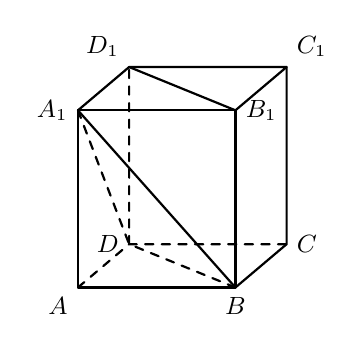
\begin{tikzpicture}[line cap=round, line join=round, thick, every node/.style={font=\small}]
  \coordinate (A) at (0,0);
  \coordinate (B) at (2,0);
  \coordinate (C) at (2.65,.55);
  \coordinate (D) at (.65,.55);
  \coordinate (A1) at (0,2.25);
  \coordinate (B1) at (2,2.25);
  \coordinate (C1) at (2.65,2.8);
  \coordinate (D1) at (.65,2.8);
  % 正方体可见外棱
  \draw (A)--(B)--(B1)--(A1)--cycle;
  \draw (A1)--(D1)--(C1)--(B1);
  \draw (B)--(C)--(C1);
  % 隐藏棱
  \draw[dashed] (A)--(D)--(C) (D)--(D1);
  % 四棱锥 A1-BB1D1D 棱
  \draw (B1)--(D1) (A1)--(B);
  \draw[dashed] (A1)--(D) (B)--(D);
  \node[below left] at (A) {$A$};
  \node[below] at (B) {$B$};
  \node[right] at (C) {$C$};
  \node[left] at (D) {$D$};
  \node[left] at (A1) {$A_1$};
  \node[right] at (B1) {$B_1$};
  \node[above right] at (C1) {$C_1$};
  \node[above left] at (D1) {$D_1$};
\end{tikzpicture}
\end{center}
\nopagebreak[4]
\Needspace{4\baselineskip}
\textbf{解析}

在正方体 $ABCD-A_1B_1C_1D_1$ 中，截面 $BB_1D_1D$ 为矩形，边长为 $BB_1=1$，$BD=\sqrt2$。
底面面积 $S_{BB_1D_1D}=1\times\sqrt2=\sqrt2$。
顶点 $A_1$ 到底面 $BB_1D_1D$ 的距离即为 $A_1$ 到对角线 $B_1D_1$ 的距离，在正方形 $A_1B_1C_1D_1$ 中此距离等于对角线长的一半，即 $h=\frac{\sqrt2}{2}$。
\Needspace{5\baselineskip}
因此四棱锥的体积为
\nopagebreak[4]
\[V=\frac13 S_{BB_1D_1D} h=\frac13\times\sqrt2\times\frac{\sqrt2}{2}=\frac13.\]

\gkanswer{答案：$1/3$}

\end{answer}
\begin{answer}
\gksolhead{12}{}

\textbf{题目}：

在平面直角坐标系中，经过三点 $(0,0),(1,1),(2,0)$ 的圆的方程为 $\underline{\qquad\qquad}$。

\Needspace{4\baselineskip}
\textbf{解析}

设圆的方程为 $x^2+y^2+Dx+Ey+F=0$。
过 $(0,0)$ 得 $F=0$；过 $(2,0)$ 得 $4+2D=0\implies D=-2$；
过 $(1,1)$ 得 $1+1-2+E=0\implies E=0$。
故圆的方程为 $x^2+y^2-2x=0$，即 $(x-1)^2+y^2=1$。

\gkanswer{答案：$(x-1)^2+y^2=1$}

\end{answer}
\begin{answer}
\gksolhead{13}{}

\textbf{题目}：

已知 $a,b\in\mathbb R$，且 $a-3b+6=0$，则 $2^a+\frac1{8^b}$ 的最小值为 $\underline{\qquad\qquad}$。

\Needspace{4\baselineskip}
\textbf{解析}

由 $a-3b+6=0$ 得 $a=3b-6$。
\Needspace{5\baselineskip}
代入原式得
\nopagebreak[4]
\[2^a+\frac1{8^b}=2^{3b-6}+2^{-3b}\geqslant 2\sqrt{2^{3b-6}\cdot 2^{-3b}}=2\sqrt{2^{-6}}=2\times\frac18=\frac14.\]
当且仅当 $3b-6=-3b\iff b=1,a=-3$ 时等号成立，故最小值为 $\frac14$。

\gkanswer{答案：$1/4$}

\end{answer}
\begin{answer}
\gksolhead{14}{}

\textbf{题目}：

\Needspace{5\baselineskip}
已知 $a\in\mathbb R$，函数
\nopagebreak[4]
\[
f(x)=\begin{cases}
x^2+2x+a-2,&x\leqslant0,\\
-x^2+2x-2a,&x>0,
\end{cases}
\]
若对任意 $x\in[-3,+\infty)$，$f(x)\leqslant|x|$ 恒成立，则 $a$ 的取值范围是 $\underline{\qquad\qquad}$。

\Needspace{4\baselineskip}
\textbf{解析}

当 $x\in[-3,0]$ 时，$|x|=-x$。不等式化为 $x^2+2x+a-2\leqslant -x\iff x^2+3x+a-2\leqslant 0$ 在 $[-3,0]$ 恒成立。
二次函数 $g(x)=x^2+3x+a-2$ 开口向上，在区间端点取最大值：
$g(-3)=a-2$，$g(0)=a-2$。
因此只需 $a-2\leqslant 0\iff a\leqslant 2$。

当 $x\in(0,+\infty)$ 时，$|x|=x$。不等式化为 $-x^2+2x-2a\leqslant x\iff x^2-x+2a\geqslant 0$ 在 $(0,+\infty)$ 恒成立。
二次函数 $h(x)=x^2-x+2a$ 的对称轴为 $x=\frac12>0$，其最小值为 $h\left(\frac12\right)=-\frac14+2a$。
因此只需 $-\frac14+2a\geqslant 0\iff a\geqslant \frac18$。

综上，$a$ 的取值范围是 $\left[\frac18,2\right]$。

\gkanswer{答案：$[1/8,2]$}

\end{answer}
\gkpart{三、解答题}

\begin{answer}
\gksolhead{15}{}

\textbf{题目}：

已知某校甲、乙、丙三个年级的学生志愿者人数分别为 240、160、160。现采用分层抽样的方法从中抽取 7 名同学去某敬老院参加献爱心活动。

(1) 应从甲、乙、丙三个年级的学生志愿者中分别抽取多少人？

(2) 设抽出的 7 名同学分别用 $A,B,C,D,E,F,G$ 表示，现从中随机抽取 2 名同学承担敬老院的卫生工作。

① 试用所给字母列举出所有可能的抽取结果；

② 设 $M$ 为事件“抽取的 2 名同学来自同一年级”，求事件 $M$ 发生的概率。

\Needspace{4\baselineskip}
\textbf{解析}

\textbf{(1) 解析} 甲、乙、丙三个年级的学生志愿者总人数为 $240+160+160=560$。
抽样比为 $\frac{7}{560}=\frac{1}{80}$。
因此：
甲年级应抽取 $240\times\frac{1}{80}=3$ 人；
乙年级应抽取 $160\times\frac{1}{80}=2$ 人；
丙年级应抽取 $160\times\frac{1}{80}=2$ 人。

\textbf{(2) 解析} ① 从 7 名同学中随机抽取 2 名同学的所有可能结果共有 $\binom72=21$ 种，具体列举如下：
$(A,B)$，$(A,C)$，$(A,D)$，$(A,E)$，$(A,F)$，$(A,G)$；
$(B,C)$，$(B,D)$，$(B,E)$，$(B,F)$，$(B,G)$；
$(C,D)$，$(C,E)$，$(C,F)$，$(C,G)$；
$(D,E)$，$(D,F)$，$(D,G)$；
$(E,F)$，$(E,G)$；
$(F,G)$。

② 不妨设 $A,B,C$ 来自甲年级，$D,E$ 来自乙年级，$F,G$ 来自丙年级。
事件 $M$（抽取的 2 名同学来自同一年级）包含的基本事件为：
来自甲年级：$(A,B)$，$(A,C)$，$(B,C)$，共 3 种；
来自乙年级：$(D,E)$，共 1 种；
来自丙年级：$(F,G)$，共 1 种。
所以事件 $M$ 包含的基本事件总数为 $3+1+1=5$ 种。
故事件 $M$ 发生的概率 $P(M)=\frac{5}{21}$。

\gkanswer{答案（1）：甲、乙、丙三个年级依次抽取 $3,2,2$ 人}

\gkanswer{答案（2）：抽取 2 名同学的所有可能结果共有 21 种；$P(M)=5/21$}

\end{answer}
\begin{answer}
\gksolhead{16}{}

\textbf{题目}：

\Needspace{5\baselineskip}
在 $\triangle ABC$ 中，内角 $A,B,C$ 所对的边分别为 $a,b,c$。已知
\nopagebreak[4]
\[
b\sin A=a\cos\left(B-\frac\pi6\right).
\]

(1) 求角 $B$ 的大小；

(2) 设 $a=2,c=3$，求 $b$ 和 $\sin(2A-B)$ 的值。

\Needspace{4\baselineskip}
\textbf{解析}

\textbf{(1) 解析} 由正弦定理 $\frac{b}{\sin B}=\frac{a}{\sin A}$ 得 $b\sin A=a\sin B$。
\Needspace{5\baselineskip}
代入已知条件 $b\sin A=a\cos\left(B-\frac\pi6\right)$，得
\nopagebreak[4]
\[a\sin B=a\cos\left(B-\frac\pi6\right).\]
因为 $a>0$，所以 $\sin B=\cos\left(B-\frac\pi6\right)=\cos B\cos\frac\pi6+\sin B\sin\frac\pi6=\frac{\sqrt3}{2}\cos B+\frac12\sin B$。
整理得 $\frac12\sin B=\frac{\sqrt3}{2}\cos B\iff\tan B=\sqrt3$。
因为 $0<B<\pi$，所以 $B=\frac\pi3$。

\Needspace{5\baselineskip}
\textbf{(2) 解析} 在 $\triangle ABC$ 中，由余弦定理得
\nopagebreak[4]
\[b^2=a^2+c^2-2ac\cos B=2^2+3^2-2\times 2\times 3\times\cos\frac\pi3=4+9-12\times\frac12=7,\]
所以 $b=\sqrt7$。

由正弦定理得 $\sin A=\frac{a\sin B}{b}=\frac{2\times\frac{\sqrt3}{2}}{\sqrt7}=\frac{\sqrt3}{\sqrt7}=\frac{\sqrt{21}}{7}$。
因为 $a=2<b=\sqrt7$，所以角 $A$ 为锐角，
从而 $\cos A=\sqrt{1-\sin^2 A}=\sqrt{1-\frac{3}{7}}=\frac{2}{\sqrt7}=\frac{2\sqrt7}{7}$。
\Needspace{5\baselineskip}
故
\nopagebreak[4]
\[\sin 2A=2\sin A\cos A=2\times\frac{\sqrt3}{\sqrt7}\times\frac{2}{\sqrt7}=\frac{4\sqrt3}{7},\]
\nopagebreak[4]
\[\cos 2A=2\cos^2 A-1=2\times\frac{4}{7}-1=\frac17.\]
\Needspace{5\baselineskip}
因此
\nopagebreak[4]
\[\sin(2A-B)=\sin 2A\cos B-\cos 2A\sin B=\frac{4\sqrt3}{7}\times\frac12-\frac17\times\frac{\sqrt3}{2}=\frac{3\sqrt3}{14}.\]

\gkanswer{答案（1）：$B=\pi/3$}

\gkanswer{答案（2）：$b=\sqrt7$，$\sin(2A-B)=3\sqrt3/14$}

\end{answer}
\begin{answer}
\gksolhead{17}{}

\textbf{题目}：

如图，在四面体 $ABCD$ 中，$\triangle ABC$ 是等边三角形，平面 $ABC\perp$ 平面 $ABD$，点 $M$ 为棱 $AB$ 的中点，$AB=2$，$AD=2\sqrt3$，$\angle BAD=90^\circ$。
\nopagebreak[4]
\begin{center}% 2018 天津文科第17题四面体示意图（据固定源第2页重绘）
\begin{tikzpicture}[line cap=round, line join=round, thick, every node/.style={font=\small}]
  \coordinate (A) at (1.2, 2.2);
  \coordinate (B) at (0, 0.6);
  \coordinate (C) at (0.8, -0.2);
  \coordinate (D) at (4.0, 1.0);
  \coordinate (M) at ($(A)!0.5!(B)$);
  % 实线可见棱
  \draw (A) -- (B) -- (C) -- cycle;
  \draw (A) -- (D) (C) -- (D);
  % 虚线不可见棱及 MD
  \draw[dashed] (B) -- (D) (M) -- (D);
  \node[above] at (A) {$A$};
  \node[left] at (B) {$B$};
  \node[below] at (C) {$C$};
  \node[right] at (D) {$D$};
  \node[above left] at (M) {$M$};
\end{tikzpicture}
\end{center}
\nopagebreak[4]
(1) 求证：$AD\perp BC$；

(2) 求异面直线 $BC$ 与 $MD$ 所成角的余弦值；

(3) 求直线 $CD$ 与平面 $ABD$ 所成角的正弦值。

\Needspace{4\baselineskip}
\textbf{解析}

\textbf{(1) 解析} 因为平面 $ABC\perp$ 平面 $ABD$，平面 $ABC\cap$ 平面 $ABD=AB$。
在平面 $ABD$ 内，已知 $\angle BAD=90^\circ$，即 $AD\perp AB$。
又 $AD\subset$ 平面 $ABD$，由面面垂直的性质定理可知，$AD\perp$ 平面 $ABC$。
因为 $BC\subset$ 平面 $ABC$，所以 $AD\perp BC$。

\textbf{(2) 解析} 取 $AB$ 的中点 $M$。因为 $\triangle ABC$ 为边长为 2 的等边三角形，所以 $CM\perp AB$，$CM=\sqrt3$。
又 $AD\perp$ 平面 $ABC$，$AD\perp AB$，$AD\perp CM$。
以 $M$ 为原点，$MB$ 所在直线为 $x$ 轴，$MC$ 所在直线为 $y$ 轴，过 $M$ 平行于 $AD$ 的直线为 $z$ 轴建立空间直角坐标系。
则各点坐标为：
$M(0,0,0)$，$B(1,0,0)$，$A(-1,0,0)$，$C(0,\sqrt3,0)$。
因为 $AD\perp AB$ 且 $AD=2\sqrt3$，所以 $D(-1,0,2\sqrt3)$。
向量 $\overrightarrow{BC}=C-B=(-1,\sqrt3,0)$，$|\overrightarrow{BC}|=2$；
向量 $\overrightarrow{MD}=D-M=(-1,0,2\sqrt3)$，$|\overrightarrow{MD}|=\sqrt{(-1)^2+0+(2\sqrt3)^2}=\sqrt{13}$。
数量积 $\overrightarrow{BC}\cdot\overrightarrow{MD}=(-1)\times(-1)+\sqrt3\times 0+0\times 2\sqrt3=1$。
\Needspace{5\baselineskip}
设异面直线 $BC$ 与 $MD$ 所成角为 $\theta$，则
\nopagebreak[4]
\[\cos\theta=\frac{|\overrightarrow{BC}\cdot\overrightarrow{MD}|}{|\overrightarrow{BC}||\overrightarrow{MD}|}=\frac{1}{2\times\sqrt{13}}=\frac{\sqrt{13}}{26}.\]

\textbf{(3) 解析} 向量 $\overrightarrow{CD}=D-C=(-1,-\sqrt3,2\sqrt3)$。
$|\overrightarrow{CD}|=\sqrt{(-1)^2+(-\sqrt3)^2+(2\sqrt3)^2}=\sqrt{1+3+12}=4$。
由题意，平面 $ABD$ 即为坐标系中的 $xz$ 平面，其法向量可取为 $\boldsymbol n=(0,1,0)$。
\Needspace{5\baselineskip}
设直线 $CD$ 与平面 $ABD$ 所成角为 $\alpha$，则
\nopagebreak[4]
\[\sin\alpha=\frac{|\overrightarrow{CD}\cdot\boldsymbol n|}{|\overrightarrow{CD}||\boldsymbol n|}=\frac{|-\sqrt3|}{4\times 1}=\frac{\sqrt3}{4}.\]

\gkanswer{答案（1）：证明见解析版}

\gkanswer{答案（2）：$\sqrt{13}/26$}

\gkanswer{答案（3）：$\sqrt3/4$}

\end{answer}
\begin{answer}
\gksolhead{18}{}

\textbf{题目}：

\Needspace{5\baselineskip}
设 $\{a_n\}$ 是等差数列，其前 $n$ 项和为 $S_n$（$n\in\mathbb N^*$），$\{b_n\}$ 是等比数列，公比大于 0，其前 $n$ 项和为 $T_n$（$n\in\mathbb N^*$）。已知
\nopagebreak[4]
\[
b_1=1,\quad b_3=b_2+2,\quad b_4=a_3+a_5,\quad b_5=a_4+2a_6.
\]

(1) 求 $S_n$ 和 $T_n$；

(2) 若 $S_n+(T_1+T_2+\cdots+T_n)=a_n+4b_n$，求正整数 $n$ 的值。

\Needspace{4\baselineskip}
\textbf{解析}

\textbf{(1) 解析} 设等比数列 $\{b_n\}$ 的公比为 $q$（$q>0$）。
由 $b_1=1$，$b_3=b_2+2$，得 $q^2=q+2\implies q^2-q-2=0$。
解得 $q=2$ 或 $q=-1$（舍去，因 $q>0$）。
所以 $b_n=2^{n-1}$，前 $n$ 项和 $T_n=\frac{1(1-2^n)}{1-2}=2^n-1$。

设等差数列 $\{a_n\}$ 的公差为 $d$。
由 $b_4=2^3=8$ 得 $a_3+a_5=2a_4=8\implies a_4=4$。
由 $b_5=2^4=16$ 得 $a_4+2a_6=16\implies 4+2a_6=16\implies a_6=6$。
公差 $d=\frac{a_6-a_4}{6-4}=\frac{6-4}{2}=1$。
首项 $a_1=a_4-3d=4-3=1$。
所以 $a_n=a_1+(n-1)d=n$。
前 $n$ 项和 $S_n=\frac{n(a_1+a_n)}{2}=\frac{n(n+1)}{2}$。

\Needspace{5\baselineskip}
\textbf{(2) 解析} 容易求得
\nopagebreak[4]
\[\sum_{k=1}^n T_k=\sum_{k=1}^n(2^k-1)=(2^1+2^2+\cdots+2^n)-n=\frac{2(1-2^n)}{1-2}-n=2^{n+1}-2-n.\]
\Needspace{5\baselineskip}
等式左边为
\nopagebreak[4]
\[S_n+\sum_{k=1}^n T_k=\frac{n(n+1)}{2}+2^{n+1}-2-n=\frac{n(n-1)}{2}+2^{n+1}-2.\]
\Needspace{5\baselineskip}
等式右边为
\nopagebreak[4]
\[a_n+4b_n=n+4\times 2^{n-1}=n+2^{n+1}.\]
\Needspace{5\baselineskip}
两边相等，得
\nopagebreak[4]
\[\frac{n(n-1)}{2}+2^{n+1}-2=n+2^{n+1}\implies\frac{n(n-1)}{2}-2=n\implies n^2-3n-4=0.\]
解得 $n=4$ 或 $n=-1$。
因为 $n\in\mathbb N^*$，所以正整数 $n$ 的值为 4。

\gkanswer{答案（1）：$S_n=n(n+1)/2$，$T_n=2^n-1$}

\gkanswer{答案（2）：$n=4$}

\end{answer}
\begin{answer}
\gksolhead{19}{}

\textbf{题目}：

设椭圆 $\frac{x^2}{a^2}+\frac{y^2}{b^2}=1$（$a>b>0$）的右顶点为 $A$，上顶点为 $B$。已知椭圆的离心率为 $\frac{\sqrt5}{3}$，$|AB|=\sqrt{13}$。

(1) 求椭圆的方程；

(2) 设直线 $l:y=kx$（$k<0$）与椭圆交于 $P,Q$ 两点，$l$ 与直线 $AB$ 交于点 $M$，且点 $P,M$ 均在第四象限。若 $\triangle BPM$ 的面积是 $\triangle BPQ$ 面积的 2 倍，求 $k$ 的值。

\Needspace{4\baselineskip}
\textbf{解析}

\textbf{(1) 解析} 椭圆右顶点为 $A(a,0)$，上顶点为 $B(0,b)$。
由 $|AB|=\sqrt{13}$ 得 $a^2+b^2=13$。
由离心率 $e=\frac ca=\frac{\sqrt5}{3}$，得 $\frac{c^2}{a^2}=\frac{a^2-b^2}{a^2}=\frac59\implies b^2=\frac49 a^2$。
代入得 $a^2+\frac49 a^2=13\implies\frac{13}{9}a^2=13\implies a^2=9$。
故 $b^2=4$。
所以椭圆方程为 $\frac{x^2}{9}+\frac{y^2}{4}=1$。

\textbf{(2) 解析} 直线 $AB$ 过点 $A(3,0)$ 与 $B(0,2)$，方程为 $\frac x3+\frac y2=1$，即 $y=-\frac23 x+2$。
联立直线 $l:y=kx$（$k<0$）与直线 $AB$，得 $kx=-\frac23 x+2\implies\left(k+\frac23\right)x=2\implies x_M=\frac{6}{3k+2}$。
因为点 $M$ 在第四象限，所以 $x_M>0$，$y_M=kx_M<0$。由 $k<0$ 知只需 $x_M>0\implies 3k+2>0\implies -\frac23<k<0$。

\Needspace{5\baselineskip}
联立直线 $l:y=kx$ 与椭圆方程 $\frac{x^2}{9}+\frac{y^2}{4}=1$，得
\nopagebreak[4]
\[\frac{x^2}{9}+\frac{k^2 x^2}{4}=1\implies(9k^2+4)x^2=36\implies x^2=\frac{36}{9k^2+4}.\]
因为点 $P$ 在第四象限，所以 $x_P=\frac{6}{\sqrt{9k^2+4}}$。
由椭圆的中心对称性，点 $Q$ 与点 $P$ 关于原点对称，故 $O$ 是 $PQ$ 的中点，$|PQ|=2|OP|$。
又 $P,Q,M$ 均在直线 $l$ 上，$\triangle BPM$ 与 $\triangle BPQ$ 在直线 $l$ 上的高相同，
故其面积之比等于底之比：$\frac{S_{\triangle BPM}}{S_{\triangle BPQ}}=\frac{|PM|}{|PQ|}$。
已知 $S_{\triangle BPM}=2S_{\triangle BPQ}$，所以 $|PM|=2|PQ|=4|OP|$。
又 $O,P,M$ 均在第四象限同一直线上，$x_O=0,x_P>0,x_M>0$，
故 $|PM|=|x_M-x_P|$，$|OP|=x_P$。
因此 $|x_M-x_P|=4x_P\implies x_M=5x_P$（$x_M=-3x_P<0$ 舍去）。
\Needspace{5\baselineskip}
代入得
\nopagebreak[4]
\[\frac{6}{3k+2}=5\times\frac{6}{\sqrt{9k^2+4}}\iff\sqrt{9k^2+4}=5(3k+2).\]
\Needspace{5\baselineskip}
两边平方得
\nopagebreak[4]
\[9k^2+4=25(9k^2+12k+4)\iff 216k^2+300k+96=0\iff 18k^2+25k+8=0.\]
因式分解得 $(2k+1)(9k+8)=0$，解得 $k=-\frac12$ 或 $k=-\frac89$。
因为 $-\frac23<k<0$，而 $-\frac89<-\frac23$ 不满足要求，必须舍去。
故 $k=-\frac12$。

\gkanswer{答案（1）：$x^2/9+y^2/4=1$}

\gkanswer{答案（2）：$k=-1/2$}

\end{answer}
\begin{answer}
\gksolhead{20}{}

\textbf{题目}：

设函数 $f(x)=(x-t_1)(x-t_2)(x-t_3)$，其中 $t_1,t_2,t_3\in\mathbb R$，且 $t_1,t_2,t_3$ 是公差为 $d$ 的等差数列。

(1) 若 $t_2=0,d=1$，求曲线 $y=f(x)$ 在点 $(0,f(0))$ 处的切线方程；

(2) 若 $d=3$，求 $f(x)$ 的极值；

(3) 若曲线 $y=f(x)$ 与直线 $y=-(x-t_2)-6\sqrt3$ 有三个互异的公共点，求 $d$ 的取值范围。

\Needspace{4\baselineskip}
\textbf{解析}

设 $t_1=t_2-d$，$t_3=t_2+d$。
令 $u=x-t_2$，则 $f(x)=u(u+d)(u-d)=u^3-d^2 u=(x-t_2)^3-d^2(x-t_2)$。
求导得 $f'(x)=3(x-t_2)^2-d^2$。

\textbf{(1) 解析} 若 $t_2=0,d=1$，则 $f(x)=x^3-x$。
切点为 $(0,f(0))=(0,0)$。
切线斜率为 $k=f'(0)=3\times 0^2-1^2=-1$。
故曲线在点 $(0,f(0))$ 处的切线方程为 $y-0=-1(x-0)$，即 $y=-x$（或 $x+y=0$）。

\textbf{(2) 解析} 若 $d=3$，则 $f(x)=(x-t_2)^3-9(x-t_2)$。
$f'(x)=3(x-t_2)^2-9=3[(x-t_2)^2-3]$。
令 $f'(x)=0$，解得 $x=t_2-\sqrt3$ 或 $x=t_2+\sqrt3$。
列表分析单调性：
当 $x<t_2-\sqrt3$ 时，$f'(x)>0$，$f(x)$ 单调递增；
当 $t_2-\sqrt3<x<t_2+\sqrt3$ 时，$f'(x)<0$，$f(x)$ 单调递减；
当 $x>t_2+\sqrt3$ 时，$f'(x)>0$，$f(x)$ 单调递增。
\Needspace{5\baselineskip}
因此，$f(x)$ 在 $x=t_2-\sqrt3$ 处取得极大值，极大值为
\nopagebreak[4]
\[f(t_2-\sqrt3)=(-\sqrt3)^3-9(-\sqrt3)=-3\sqrt3+9\sqrt3=6\sqrt3;\]
\Needspace{5\baselineskip}
在 $x=t_2+\sqrt3$ 处取得极小值，极小值为
\nopagebreak[4]
\[f(t_2+\sqrt3)=(\sqrt3)^3-9(\sqrt3)=3\sqrt3-9\sqrt3=-6\sqrt3.\]

\Needspace{5\baselineskip}
\textbf{(3) 解析} 曲线 $y=f(x)$ 与直线 $y=-(x-t_2)-6\sqrt3$ 的公共点横坐标满足方程
\nopagebreak[4]
\[(x-t_2)^3-d^2(x-t_2)=-(x-t_2)-6\sqrt3.\]
令 $u=x-t_2$，方程化为 $u^3-(d^2-1)u+6\sqrt3=0$。
设 $g(u)=u^3-(d^2-1)u+6\sqrt3$。
原曲线与直线有三个互异公共点，等价于方程 $g(u)=0$ 有三个互异实根。
求导得 $g'(u)=3u^2-(d^2-1)$。
若 $d^2-1\leqslant 0$，则 $g'(u)\geqslant 0$，$g(u)$ 在 $\mathbb R$ 上单调递增，最多只有一个实根，不合题意。
因此必须 $d^2-1>0$。
令 $g'(u)=0$，得极值点 $u_1=-\sqrt{\frac{d^2-1}{3}}$，$u_2=\sqrt{\frac{d^2-1}{3}}$。
此时 $g(u)$ 在 $u_1$ 处取得极大值，在 $u_2$ 处取得极小值。
\Needspace{5\baselineskip}
方程 $g(u)=0$ 有三个互异实根的充要条件是极大值为正且极小值为负，即
\nopagebreak[4]
\[g\left(\sqrt{\frac{d^2-1}{3}}\right)<0\quad\text{\text{且}}\quad g\left(-\sqrt{\frac{d^2-1}{3}}\right)>0.\]
\Needspace{5\baselineskip}
计算极小值：
\nopagebreak[4]
\[g\left(\sqrt{\frac{d^2-1}{3}}\right)=\left(\sqrt{\frac{d^2-1}{3}}\right)^3-(d^2-1)\sqrt{\frac{d^2-1}{3}}+6\sqrt3=-\frac23(d^2-1)\sqrt{\frac{d^2-1}{3}}+6\sqrt3<0,\]
\Needspace{5\baselineskip}
即
\nopagebreak[4]
\[\frac23(d^2-1)\sqrt{\frac{d^2-1}{3}}>6\sqrt3\iff (d^2-1)\sqrt{\frac{d^2-1}{3}}>9\sqrt3\iff\left(\frac{d^2-1}{3}\right)^{\frac32}>3\sqrt3=3^{\frac32}.\]
两边平方得 $\left(\frac{d^2-1}{3}\right)^3>27\implies \frac{d^2-1}{3}>3\implies d^2-1>9\implies d^2>10$。
当 $d^2>10$ 时，易验极大值 $g(u_1)=\frac23(d^2-1)\sqrt{\frac{d^2-1}{3}}+6\sqrt3>0$ 恒成立。
由 $d^2>10$ 解得 $d>\sqrt{10}$ 或 $d<-\sqrt{10}$。
因此，$d$ 的取值范围是 $(-\infty,-\sqrt{10})\cup(\sqrt{10},+\infty)$。

\gkanswer{答案（1）：$y=-x$}

\gkanswer{答案（2）：极大值为 $6\sqrt3$，极小值为 $-6\sqrt3$}

\gkanswer{答案（3）：$(-\infty,-\sqrt{10})\cup(\sqrt{10},+\infty)$}

\end{answer}